\section{COCOMO analysis}
The COCOMO model allows to estimate the time effort required by the project. We use the version of this model called COCOMO II. It is based on a main formula:
\begin{equation}
PM = A * Size^{E} * \prod_{1<=i<=n}^{} EM_{i} 
\end{equation}

where:
\begin{itemize}
\item \textbf{PM} stands for "Person-Months
\item \textbf{A}=2.94. It approximates a productivity constant in PM/KSLOC for the case where E = 1.0.
\item \textbf{Size} is measured in KSLOC and is the result of the Function Points analysis.
\item \textbf{E} is an aggregation of 5 \textbf{scale factors}:
	\begin{itemize}[label = {-}]
	\item \textbf{Precedentedness:} It is high if the project is similar to several previous projects
	\item \textbf{Development Flexibility:} It is high if there are no specific constraints to conform to pre-established 		requirements and external interface specifications.
	\item \textbf{Architecture / Risk Resolution:}It is high if the project plan includes a good risk management plan, a clear definition of budget and schedule, with a focus on architectural definition
\item \textbf{Team Cohesion:}It is high if all stakeholders are able to work in a team and share the same vision and commitment.
\item \textbf{Process Maturity:} Refers to a well known method for assessing the maturity of a software organization, CMMI, that is a process level improvement training and appraisal program.
	\end{itemize}
\begin{figure}[H]	
	\centering
	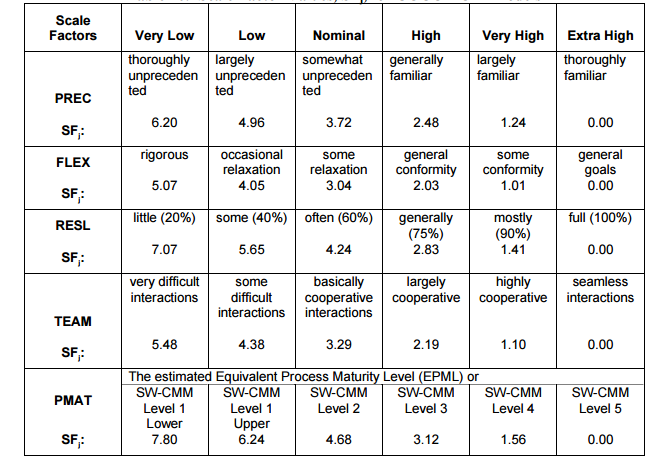
\includegraphics[scale = 0.7]{img/scaleFactors.png}
	\caption{Scale Factors}
\end{figure}

E is calculated with the formula:
\begin{equation}
E = B + 0.01 * \sum_{1<=j<=5}^{} SF_{j}
\end{equation}
where B=0.91

\item \textbf{EM} stands for Effort Multiplier. Effort multipliers are derived from \textbf{Cost drivers}. The selection of these cost drivers depends on wh1ether the project regards a \textbf{Post-Architecture} system or a \textbf{Early Design} system. We are in the Early Design case, because we are extending an existing product and our system will be developed from scratch. So the cost drivers are:
\begin{itemize}[label = {-}]
\item Personnel Capability (PERS): it is a combination of Analyst Capability(ACAP), Programmer Capability(PCAP) and Personnel Continuity cost driver of Post-Architecture.
\begin{figure}[H]	
	\centering
	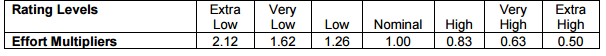
\includegraphics[scale = 0.6]{img/PERS.png}
	\caption{EMs of PERS}
\end{figure}
\item Product Reliability and Complexity(RCPX): it is a combination of Required Software Reliability(RELY), Data Base Size(DATA), Product Complexity(CPLX) and Documentation Match to Lif-Cycle Need(DOCU) cost drivers of Post-Architecture. 
\begin{figure}[H]	
	\centering
	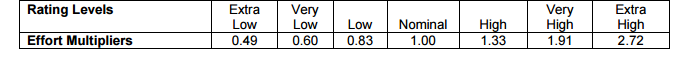
\includegraphics[scale = 0.6]{img/RCPX.png}
	\caption{EM of RCPX}
\end{figure}
\item Developed for Reusability(RUSE)
\begin{figure}[H]	
	\centering
	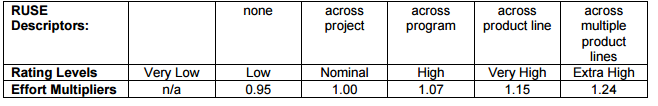
\includegraphics[scale = 0.6]{img/RUSE.png}
	\caption{EMs of RUSE}
\end{figure}

\item Platform Difficulty(PDIF): it is a combination of Execution Time Constraint(TIME), Main Storage Constraint(STOR) and Platform Volatility(PVOL) cost drivers of Post-Architecture. 
\begin{figure}[H]	
	\centering
	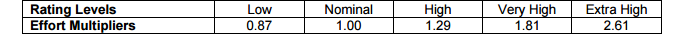
\includegraphics[scale = 0.6]{img/PDIF.png}
	\caption{EMs of PDIF}
\end{figure}

\item Personnel Experience(PREX): it is a combination of Application Experience(APEX), Platform Experience(PLEX), Language and Tool Experience(LTEX) cost drivers of Post-Architecture. 
\begin{figure}[H]	
	\centering
	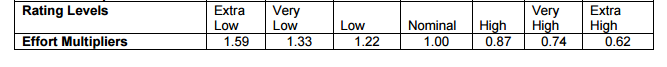
\includegraphics[scale = 0.6]{img/PREX.png}
	\caption{EMs of PREX}
\end{figure}

\item Facilities(FCIL):it is a combination of Use of Software Tools(TOOL) and Multisite Development(SITE) cost drivers of Post-Architecture. 

\begin{figure}[H]	
	\centering
	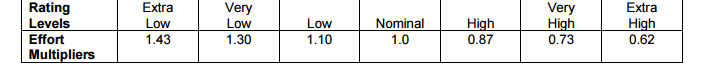
\includegraphics[scale = 0.6]{img/FCIL.png}
	\caption{EMs of FCIL}
\end{figure}

\item Required Development Schedule(SCED)

\begin{figure}[H]	
	\centering
	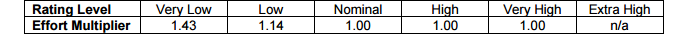
\includegraphics[scale = 0.6]{img/SCED.png}
	\caption{EMs of SCED}
\end{figure}

\end{itemize} 
\end{itemize}


